\documentclass[a4paper,12pt,twoside]{report}
\usepackage[english]{babel}
\usepackage[utf8]{inputenc}
\pagestyle{headings}
\author{Luis Carlos Garcia-Peraza Herrera}
\date{\today}
\usepackage{graphicx}
\usepackage{listings}

\begin{document}
\chapter*{Conway's Game of Life Coursework}
\section*{Conway's Game of Life Explanation (Q1)}
	
Game of Life is a cellular automata designed by Conway in 1970. It is a zero-player game and the only input provided is the initial state of the game board.
The state of the board is updated at each iteration of the game in a cell-by-cell basis. The decision of the state of each cell in the next iteration depends
on the number of cells that are alive in its 8-neighbourhood and on the state of each cell in particular. Therefore:
\newline\newline
1) If a cell is alive and has exactly two or three neighbours alive it will be alive in the next iteration. Otherwise, it dies.
\newline\newline
2) If a cell is dead and has exactly three neighbours alive it will be alive in the next iteration. Otherwise, it remains dead.

\section*{Build Instructions}
\$ ./build.sh
\section*{Code Organisation}
The code has been organised in several folders: \newline
- inc: contains the header files (.h or .hpp). \newline
- src: contains the code files (.c or .cpp). \newline
- test: contains all the required headers and code files for the unit tests (i.e. catch and test.cpp, which is the file that contains all the tests). \newline
- doc: contains all the documentation of the project including this report. \newline
- bin: contains the two binary files produced by this project, the app and the tests.
\section*{Run Unit Tests}
Execute the following commands in the main directory of the project in order to check the correctness of the code. \newline
\newline
\$ ./test.sh
\section*{Run the Program}
After the program and the tests have been compiled, execute this command to run the program:
\newline
\$ ./run.sh \newline
\$ build/src/GameOfLife --input test/input.txt --output output.txt --niter 100\newline
\$ build/src/GameOfLife --random 100 --output output.txt --niter 100
\section*{Parallelisation}
The code has been parallelised using OpenMP. The part of the code that has been parallelised is the method evolve() of the Board class since each cell is updated  based exclusively on the previous state of the cells in its neighbourhood, which does not change while the other cells are being updated.
\begin{lstlisting}

// Code that executes Conway's rules and updates the board
#pragma omp parallel for
for (uint32_t i = 0; i < m_rows; i++) {
   for (uint32_t j = 0; j < m_cols; j++) {
      uint32_t nAlive = aliveNeighbours(i, j);
      if (m_board[i][j].isAlive()) { // If cell is alive
         if (nAlive == 2 || nAlive == 3)
            newBoard.cell(i, j, true);
         else
            newBoard.cell(i, j, false);
	  }
	  else {                         // If cell is not alive
         if (nAlive == 3)
            newBoard.cell(i, j, true);
         else
            newBoard.cell(i, j, false);
      }
   }
}
\end{lstlisting}
\section*{Results}
Video uploaded to YouTube demonstrating Game of Life:
\newline\newline
\textit{https://www.youtube.com/watch?v=949ciYmRyhE}
\newline\newline
This video has been generated running this program with the following command:
\newline\newline
\$ ./GameOfLife --random 100 --niter 500 --output output.txt
\newline\newline
Then, the file output.txt is converted into a video with the following command:
\newline\newline
\$ python extras/txt\_to\_video.py output.txt video.mp4
\newline\newline
\underline{Speed tests comparing the execution time with and without OpenMP:}
\newline\newline
\textbf{OS}                : MAC OS X 10.9.5 \newline
\textbf{Machine}           : Intel Core i7 2.5GHz 16GB 1600MHz DDR3 (4 cores) \newline
\textbf{Benchmark}         : Unix 'time' command \newline
\textbf{Iterations}        : 100 \newline
\textbf{Board sizes tested}: 100x100, 1000x1000, 2000x2000 \newline
\newline
Each test has been executed three times.
\newline\newline
\underline{Without OpenMP:}
\newline\newline
GameOfLife -r 100 -n 100 -o output.txt  0.27s user 0.02s system 99\% cpu 0.294 total \newline
GameOfLife -r 100 -n 100 -o output.txt  0.27s user 0.01s system 99\% cpu 0.286 total \newline
GameOfLife -r 100 -n 100 -o output.txt  0.28s user 0.01s system 99\% cpu 0.293 total \newline
\newline
GameOfLife -r 1000 -n 100 -o output.txt  26.30s user 0.37s system 99\% cpu 26.676 total \newline
GameOfLife -r 1000 -n 100 -o output.txt  26.68s user 0.39s system 99\% cpu 27.066 total \newline
GameOfLife -r 1000 -n 100 -o output.txt  26.54s user 0.39s system 99\% cpu 26.936 total \newline
\newline
GameOfLife -r 2000 -n 100 -o output.txt  105.65s user 1.52s system 99\% cpu 1:47.20 total \newline
GameOfLife -r 2000 -n 100 -o output.txt  106.05s user 1.57s system 99\% cpu 1:47.67 total \newline
ameOfLife -r 2000 -n 100 -o output.txt  105.97s user 1.58s system 99\% cpu 1:47.57 total \newline
\newline
\underline{With OpenMP:} \newline
\newline
GameOfLife -r 100 -n 100 -o output.txt  0.50s user 0.02s system 375\% cpu 0.138 total \newline
GameOfLife -r 100 -n 100 -o output.txt  0.50s user 0.02s system 356\% cpu 0.147 total \newline
GameOfLife -r 100 -n 100 -o output.txt  0.50s user 0.02s system 382\% cpu 0.138 total\newline
\newline
GameOfLife -r 1000 -n 100 -o output.txt  60.73s user 0.44s system 570\% cpu 10.729 total \newline
GameOfLife -r 1000 -n 100 -o output.txt  60.02s user 0.43s system 564\% cpu 10.714 total \newline
GameOfLife -r 1000 -n 100 -o output.txt  62.75s user 0.44s system 568\% cpu 11.124 total \newline
\newline
GameOfLife -r 2000 -n 100 -o output.txt  282.59s user 1.80s system 607\% cpu 46.848 total \newline
GameOfLife -r 2000 -n 100 -o output.txt  284.56s user 1.79s system 611\% cpu 46.810 total \newline
GameOfLife -r 2000 -n 100 -o output.txt  286.03s user 1.82s system 611\% cpu 47.105 total \newline
\newline
\underline{Summary (without OpenMP):} \newline \newline
100x100:	0.294s,	 0.286s,  0.293s \newline
1000x1000: 26.676s, 27.066s, 26.936s \newline
2000x2000: 107.20s, 107.67s, 107.57s \newline
\newline
\underline{Summary (with OpenMP):} \newline \newline
100x100:    0.138s,  0.147s,  0.138s \newline
1000x1000: 10.729s, 10.714s, 11.124s \newline
2000x2000: 46.848s, 46.810s, 47.105s \newline
\newline
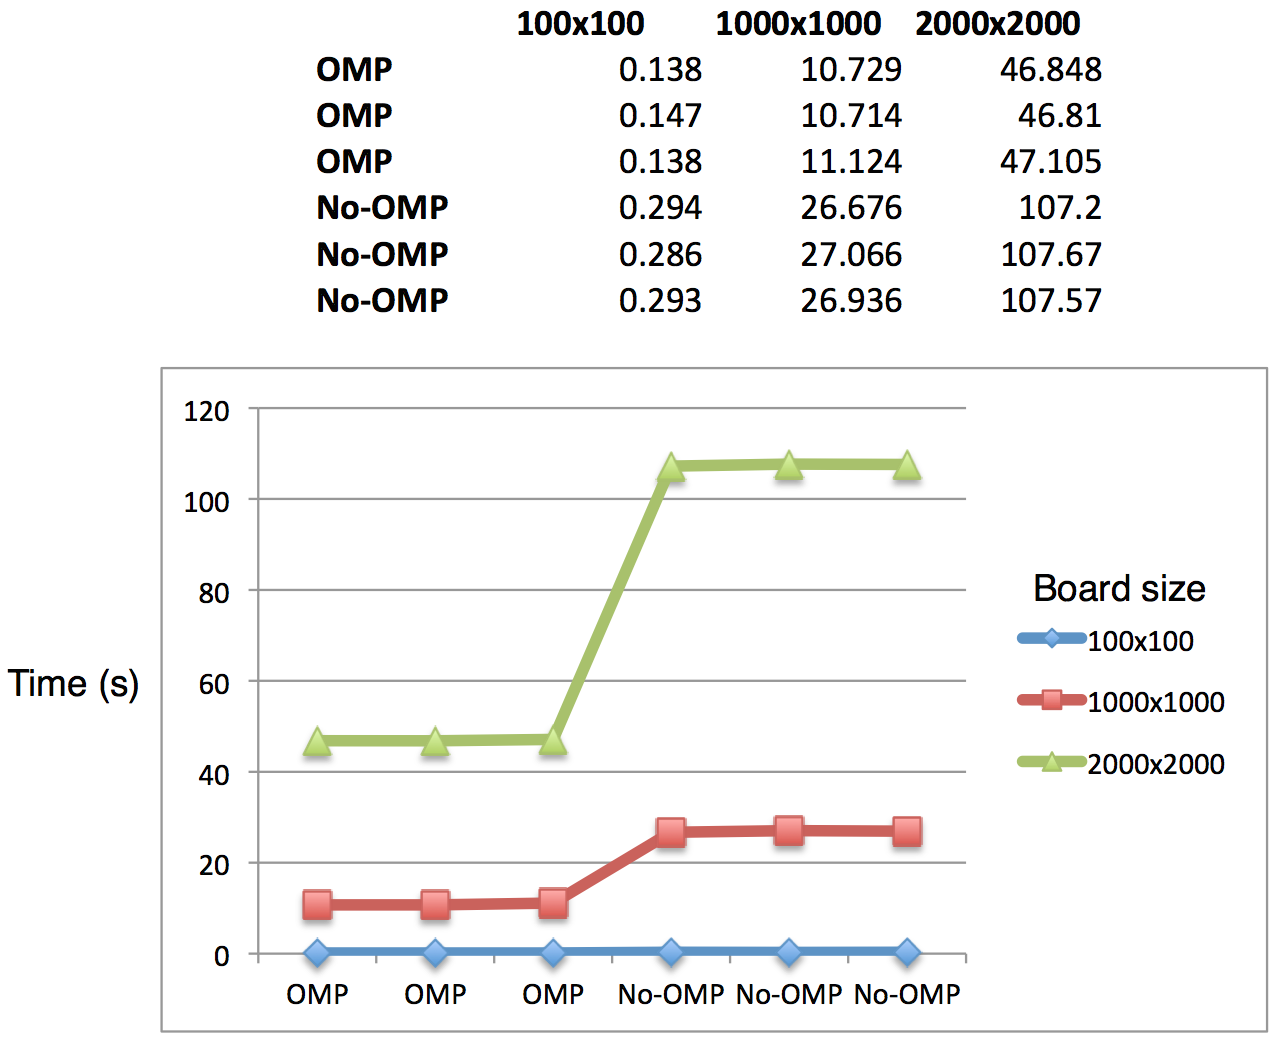
\includegraphics[width=300pt]{graph.png}

\section*{Conclusions}

The speedup achieved with OpenMP for a boards of 100x100, 1000x1000 and 2000x2000 are 206.38\%, 299.99\% and 229.07\% respectively.

\end{document}
